\section{Introdução}

O experimento apresentado neste relatório consistiu em avaliar a influência de dois parâmetros básicos no tempo de queda de alguns modelos de "helicóptero" feito em dobraduras de papel.

\subsection{\textit{Six Sigma}}

A filosofia \textit{Six Sigma} (ou Seis Sigma) é uma estratégia em que você define rotinas e desenvolve trabalhos de melhoria de processos em sua organização \cite{sixsigma}. Este método foi originado pelo programa de melhoria da qualidade da Motorola em 1987 com o objetivo de se aproximar do zero defeito. Com o sucesso alcançado pela metodologia na empresa, o processo foi difundido \cite{correa}. \textit{Six Sigma} trabalha com três grandes objetivos: redução de custos, otimização de processos e satisfação do cliente \cite{sixsigma}.

Tendo em vista essa informação, existe uma escala que determina a qualidade do processo:

\begin{figure}[h]
  \centering
  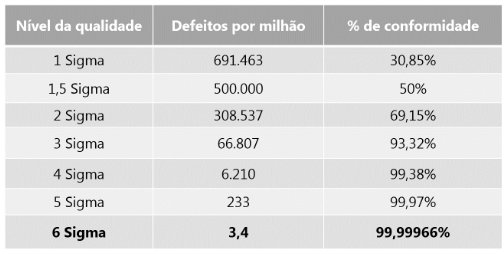
\includegraphics[scale=0.7]{images/tabless.png}
  \caption{Tabela Six Sigma \cite{sixsigma}}
  \label{fig:sixsigma}
\end{figure}

A partir da tabela, podemos perceber o espectro de algumas empresas, que trabalham em produção de milhões de unidades, então obter somente 99\% de confiabilidade não é o bastante. O processo é definido como 6 Sigma ao atingir uma proporção de 3 ou 4 erros a cada 1 milhão de unidades produzidas. Algumas empresas aceitam trabalhar como 4 Sigma em alguns dos seus processos.

\subsection{Otimização de Processos}

A otimização de respostas em um processo é fundamental para o \textit{Six Sigma} na fase de melhoria. Uma das ferramentas mais importantes que representa o conceito principal dessa filosofia é a Otimização de Processos (DoE). A DoE busca combinar fatores de um processo com o objetivo de otimizar a resposta desejada extraindo o máximo possível de informações com um número mínimo de experimentos. \cite{abepro}

O planejamento e a condução desses testes também fazem parte do DoE, visto que a falta de planejamento ou a má condução pode culminar em resultados incoerentes, obrigando a repetição de todo o processo de análise, ou mesmo falsos-positivos. Os testes devem ser projetados de modo que a aleatoriedade esteja sempre presente, em detrimento a qualquer eventual manipulação dos dados, pois ela é uma peça fundamental na normalidade dos experimentos.